\begin{frame} % 什么是移动机器人?
\frametitle{Background}

\begin{columns}
\column{0.5\textwidth}
\begin{figure}
    \centering
    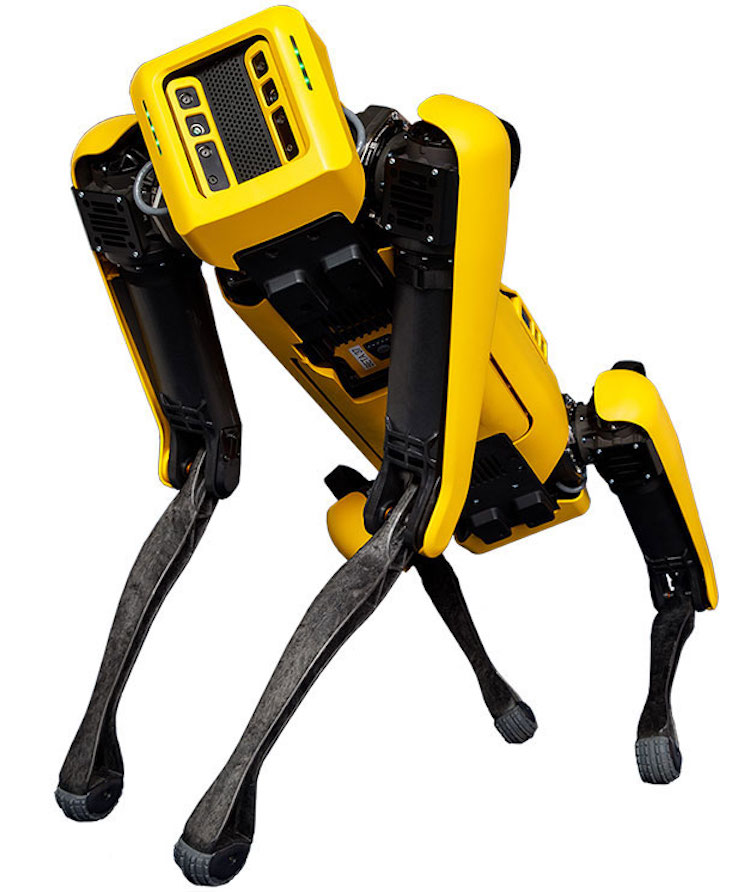
\includegraphics[width=2cm]{photos/boston-dynamics-spot.jpg} 
    \vspace{-0.3cm}
    \caption{Spot from Boston Dynamics}
    \label{fig:spot}
    \vspace{-0.7cm}
\end{figure}

\begin{figure}
    \centering
    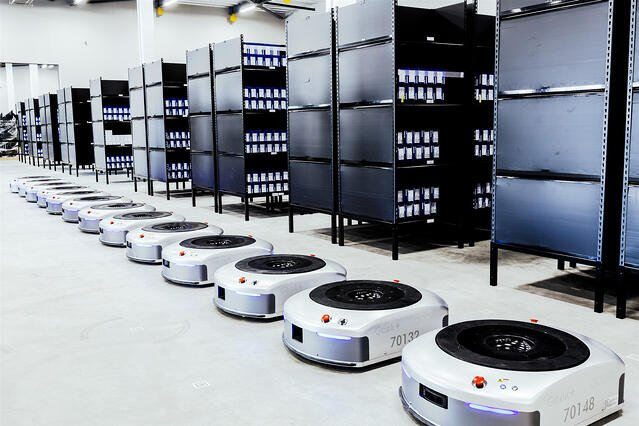
\includegraphics[width=3.2cm]{photos/Geek+ Picking.jpg}
    \vspace{-0.3cm}
    \caption{AGV from Geek+}
    \vspace{-0.7cm}
    \label{fig:geekplus}
\end{figure}

\begin{figure}
    \centering
    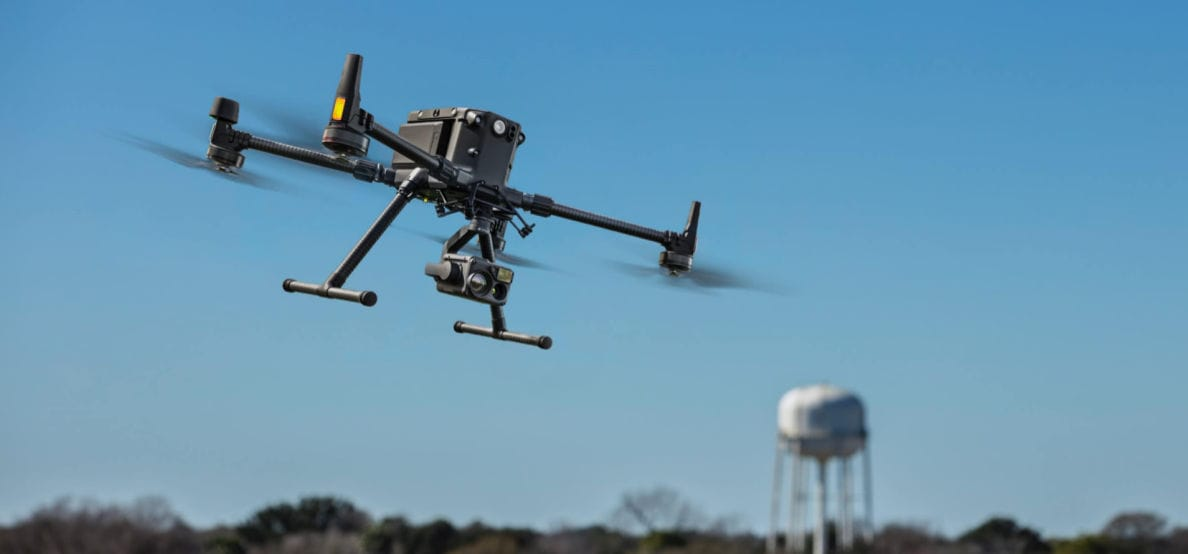
\includegraphics[width=3.2cm]{photos/dji.jpg}
    \vspace{-0.3cm}
    \caption{Quadrotor from DJI}
    \label{fig:grass}
\end{figure}

\column{0.5\textwidth}
% 什么是移动机器人?

\textbf{What is a mobile robot?}
\begin{itemize}
    \item A robot that can move itself to point A from point B. 
\end{itemize}

\textbf{Many mobile robots have been developed, it can be divided into: }
\begin{itemize}
    \item Legged mobile robots
    \item Wheeled mobile robots
    \item Aerial mobile robots
    \item ...
\end{itemize}
\end{columns}
\end{frame}

\begin{frame} % 移动机器人所处的环境是怎么样的?
\frametitle{Background}
\begin{columns}
\column{0.5\textwidth}
\begin{figure}
    \centering
    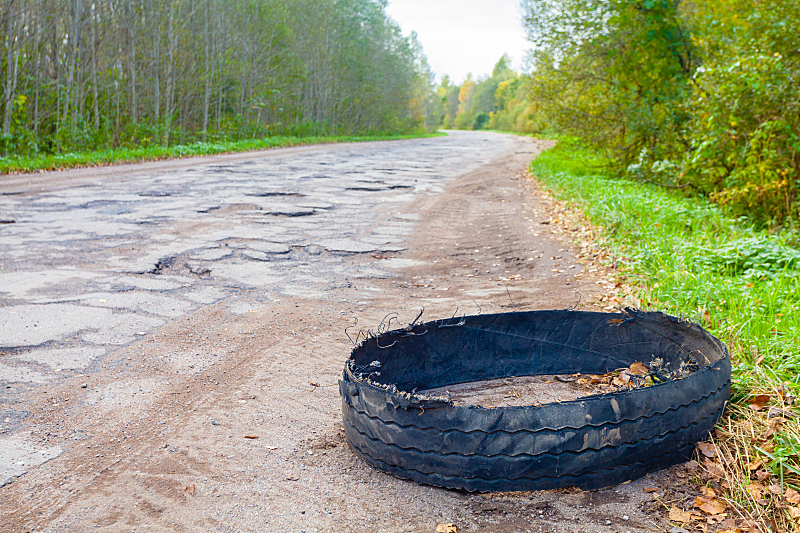
\includegraphics[width=4.6cm]{photos/rough-terrain.jpg} 
    \vspace{-0.3cm}
    \caption{Rough road}
    \label{fig:rough-terrain}
    \vspace{-0.7cm}
\end{figure}

\begin{figure}
    \centering
    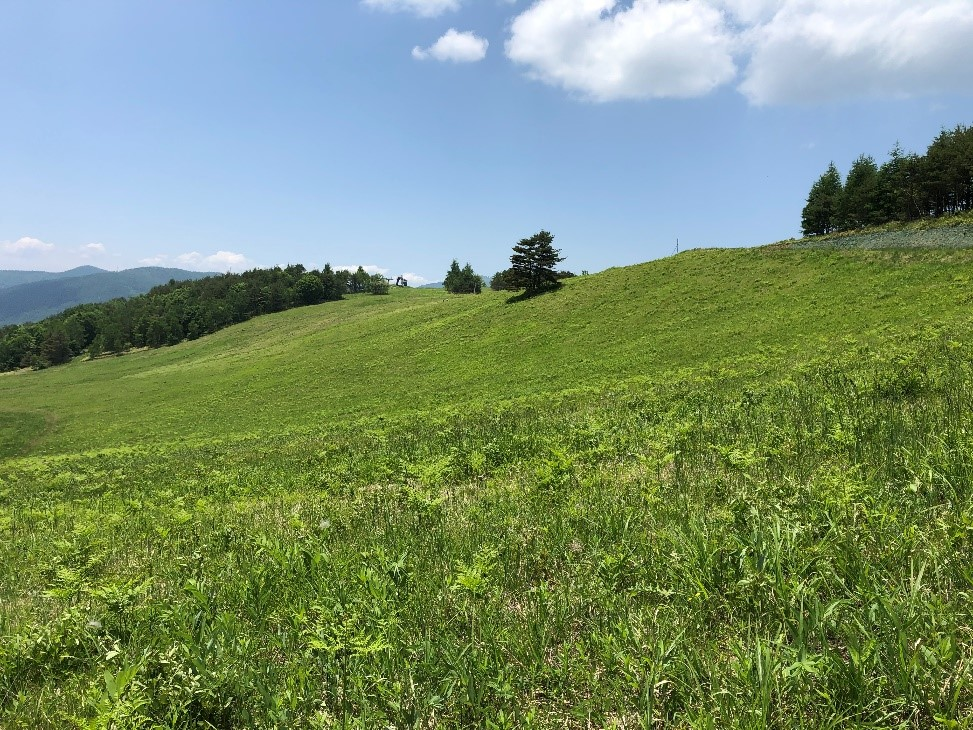
\includegraphics[width=4.6cm]{photos/草地.png}
    \vspace{-0.3cm}
    \caption{Grassland}
    \label{fig:grass-road}
\end{figure}

\column{0.5\textwidth}
\textbf{Road characteristics:}
% 特点:有一定的崎岖路面(可通过的障碍高度<15cm)、hard、
\begin{itemize}
    \item Rough \\(Obstacle height $<$ 15cm)
    \item Hard
    \item Not smooth
\end{itemize}
\textbf{Mobility requirements for a ground mobile robot in outdoors:}
% 移动能力、越障能力
\begin{itemize}
    \item Overcome complex environments
    \item Maintain stability
    \item Agile locomotion ($>1 body/s$) \\(Complete tasks on time)
\end{itemize}
\end{columns}
\end{frame}